\begin{figure}[t]
\centering
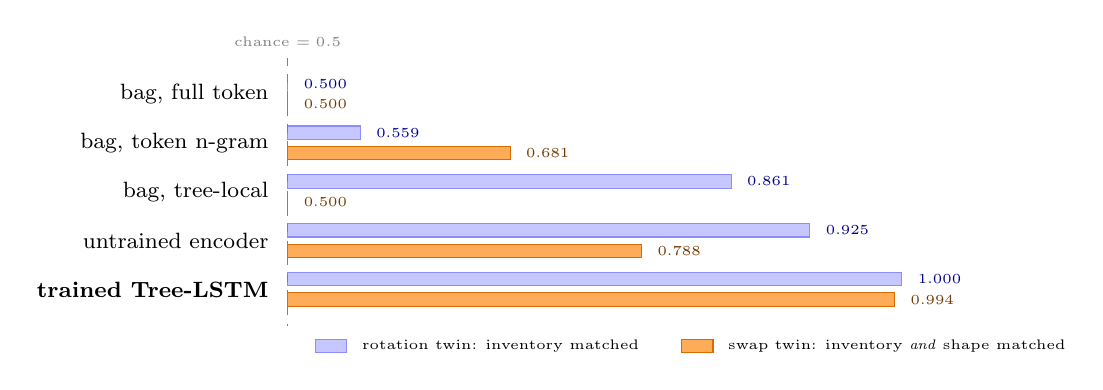
\begin{tikzpicture}[font=\small]

\def\SC{7.8}     % x-length for the range [0.5, 1.0]
\def\bh{0.17}    % bar height
\def\dy{0.62}    % row pitch

% rows: i / rotation value / swap value / label
\foreach \i/\rot/\swp/\lbl in {
  0/0.500/0.500/{bag, full token},
  1/0.559/0.681/{bag, token n-gram},
  2/0.861/0.500/{bag, tree-local},
  3/0.925/0.788/{untrained encoder},
  4/1.000/0.994/{\textbf{trained Tree-LSTM}}}
{
  \pgfmathsetmacro{\yy}{-\i*\dy}
  \pgfmathsetmacro{\wr}{(\rot-0.5)/0.5*\SC}
  \pgfmathsetmacro{\ws}{(\swp-0.5)/0.5*\SC}
  \node[anchor=east, font=\footnotesize] at (-0.12, \yy) {\lbl};
  % rotation twin (upper, light)
  \fill[blue!22] (0, \yy+0.045) rectangle (\wr, \yy+0.045+\bh);
  \draw[blue!45] (0, \yy+0.045) rectangle (\wr, \yy+0.045+\bh);
  \node[anchor=west, font=\tiny, blue!55!black] at (\wr+0.08, \yy+0.045+\bh/2) {\rot};
  % swap twin (lower, dark)
  \fill[orange!65] (0, \yy-0.045-\bh) rectangle (\ws, \yy-0.045);
  \draw[orange!85!black] (0, \yy-0.045-\bh) rectangle (\ws, \yy-0.045);
  \node[anchor=west, font=\tiny, orange!45!black] at (\ws+0.08, \yy-0.045-\bh/2) {\swp};
}

% chance line
\draw[dashed, gray] (0, 0.46) -- (0, -4*\dy-0.46);
\node[font=\tiny, gray, anchor=south] at (0, 0.48) {chance $=0.5$};

% legend
\fill[blue!22] (0.35, -4*\dy-0.80) rectangle (0.75, -4*\dy-0.64);
\draw[blue!45] (0.35, -4*\dy-0.80) rectangle (0.75, -4*\dy-0.64);
\node[anchor=west, font=\tiny] at (0.82, -4*\dy-0.72)
  {rotation twin: inventory matched};
\fill[orange!65] (5.0, -4*\dy-0.80) rectangle (5.4, -4*\dy-0.64);
\draw[orange!85!black] (5.0, -4*\dy-0.80) rectangle (5.4, -4*\dy-0.64);
\node[anchor=west, font=\tiny] at (5.47, -4*\dy-0.72)
  {swap twin: inventory \emph{and} shape matched};

\end{tikzpicture}
\caption{\textbf{What can solve the twin probe, and what happens when you close the shape
loophole.} Each held-out form on EQNET \texttt{poly8} is paired with a twin of identical token and
operator multisets ($K{=}500$; chance $0.5$; tags \texttt{r72}, \texttt{r73}). Under the
\emph{rotation} twin (blue) inventory is matched but local shape is not, and the tree-local bag
scores $0.861$, so that probe cannot attribute the encoder's margin to composition. Under the
\emph{swap} twin (orange) a sibling exchange leaves the tree-local bag \emph{exactly} invariant, so
both inventory and shape are pinned at $0.500$ by construction. Closing the loophole costs the
untrained encoder $0.925 \to 0.788$ while the trained encoder holds at $0.994$: the trained--untrained
gap \emph{widens} from $0.075$ to $0.206$.}
\label{fig:tiers}
\end{figure}
